\documentclass[a4paper,twocolumn,nobalancelastpage]{revtex4-1}
\usepackage{amsmath,amssymb,graphicx,hyperref,mathtools, color}
\usepackage{sidecap}
\usepackage{subcaption}
\usepackage[labelfont=bf]{caption}
\usepackage[labelsep=space]{caption}
\usepackage[font={small}]{caption}
\usepackage{float}

\newcommand{\vect}[1]{\mathbf{#1}}
\newcommand{\tvr}{\tilde{\vect{r}}}
\newcommand{\tvrp}{\tilde{\vect{r}}^\prime}
\newcommand{\lho}{l_{HO}}
\newcommand{\wz}{w(z_0)}
\newcommand{\wzsq}{w^2(z_0)}
\newcommand{\af}{\psi_{\nu\mu}}
\newcommand{\afp}{\psi_{\nu'\mu'}}
\newcommand{\lf}{\alpha_{nm}}
\newcommand{\lfp}{\alpha_{n'm'}}
\newcommand{\chiaf}{\chi_{\nu,\mu}^L\left(\frac{r}{\lho}\right)}
\newcommand{\chiafp}{\chi_{\nu',\mu'}^L\left(\frac{r}{\lho}\right)}
\newcommand{\chilf}{\chi_{n,m}^L\left(\frac{\sqrt{2}r}{w(z_0)}\right)}
\newcommand{\chilfp}{\chi_{n,m}^L\left(\frac{\sqrt{2}r}{w(z_0)}\right)}
\newcommand{\intfour}{\mathcal{I}nt[\chi^4]}


\DeclarePairedDelimiter\abs{\lvert}{\rvert}

\graphicspath{{./figures/}{./figures/realspace/}{./figures/modespace/}}

\begin{document}

\section{Equations of motion}
\label{sec:eom-general}

We consider a longitudinally pumped cavity with a Bose-condensed cloud of atoms. We assume the BEC is confined in the z-direction, in the separable form $\Psi(x,y,z)=\psi(x,y)Z(z)$. 
We consider the in-plane motion of the atoms, which obey the equation of motion:

\begin{multline}
\label{eq:eqnpsifirst}
i\hbar \partial_t \psi(\vect{r})= -\frac{\hbar^2 \nabla^2}{2m_a}\psi(\vect{r})+ \frac{m_a \omega_T^2}{2} \vect{r}^2 \psi(\vect{r}) \\ - \mathcal{E}_0 
\int \, \mathrm{d}z |Z(z)|^2|\varphi(\vect{r},z)|^2 \psi(\vect{r})
\end{multline}

where $m_a$ is the mass of the atoms, $\omega_T$ is the oscillator trap frequency, $\mathcal{E}_0$ is the shift due to the photon population, and the three-dimensional light field can be written as:

\begin{equation}
\label{eq:fulllightfield}
\varphi(x,y,z)= \sum_{n,m,q} \alpha_{nmq} u_{nmq}(x,y,z)
\end{equation}

where m, n label transverse modes and q labels the longitudinal modes. Note that $q$ is not completely free: in the confocal and near-confocal case we consider, the index $q$ relates to the $q$ of the fundamental mode $q_0$ and the m,n indeces as $2q+m+n=2 q_0$. This yields the condition that $m$ and $n$ must have the same parity, and $q$ is then fully determined by the other two indeces and can be dropped. We will restrict ourselves to even modes for which $m+n$ is even.

Note that $u_{n,m}$ as defined below has units of 1/L, and since the $\alpha_{nm}$ are dimensionless this means that $\mathcal{E}_0$ has units of energy times area, and the light field $\varphi(\vect{r},z)$ also has units of 1/L. 

The three-dimensional light equation of motion reads: 

\begin{widetext}

\begin{multline}
\label{eq:eqnalphafirst}
 i\partial_t \alpha_{nm}=(\omega_{n,m}-\omega_{pump}-i\kappa)\alpha_{n,m}+f_{n,m} \\ \qquad - \mathcal{E}_0 N \sum_{n',m'} \int \int \mathrm{d}^2\vect{r} \mathrm{d}z |Z(z)|^2 |\psi(\vect{r})|^2 u^*_{m,n}(\vect{r},z) u_{m',n'}(\vect{r},z)\alpha_{m',n'}
\end{multline}

\end{widetext}

where we have taken $\hbar=1$, and therefore here the units of $\mathcal{E}_0$ are really frequency. 

The pump term in eq. \ref{eq:eqnalphafirst} is defined as:

\begin{equation}
\label{eq:pumptermdef}
  f_{m,n} = \int d^2\vect{r} f(\vect{r}) u^\ast_{m,n,q}(\vect{r}, - z_R),
\end{equation}

where $f(\vect{r})$ is the spatial profile of the pump in units of frequency over length (or root area). We will assume this takes a Gaussian form

\begin{displaymath}
\label{eq:gaussianpump}
f(\vect{r})=f_P e^{\frac{\vec{r}^2}{2 \sigma_P^2}}
\end{displaymath}

where $f_P$ is the pump intensity parameter, absorbing the normalisation factors, and $\sigma_P$ is the pump width.

\subsection{Basis functions}
\label{sec:basisfunction}

In solving the above, we may choose to work either with Gauss-Hermite or Gauss-Laguerre modes.  For numerics, Laguerre is preferable as it allows us to consider the radially symmetric case efficiently. Hermites are easier to do analytically.

In the Hermite case we will consider:

\begin{multline}
  u_{m,n}(x,y,z) = 
  \frac{1}{w(z)}
  \chi_n\left( \frac{\sqrt{2} x}{w(z)} \right)
  \chi_m\left( \frac{\sqrt{2} y}{w(z)} \right)
  \\
  \cos \left[
    k \left( z + \frac{r^2}{2R(z)} \right) - (m+n+1) \psi(z) + \xi_{q} \right],
\end{multline}

where the beam waist $w(z)$, radius of curvature $R(z)$ and Guoy phase $\psi(z)$ are discussed in the appendix \ref{sec:gaussian-optics}. The $\xi_q$ term does not really need a $q$ defined since, as discussed above, we can get $q$ entirely from $m, n$ and $q_0$.

The functions $\chi_n(x)$ are normalised Gauss-Hermite functions, i.e.

\begin{displaymath}
  \chi_n(x) = \sqrt[4]{\frac{2}{\pi}}
  \frac{1}{\sqrt{2^n n!}} H_n(x) \exp\left(-\frac{x^2}{2} \right).
\end{displaymath}

In the Laguerre case we instead have:

\begin{multline}
  u_{m,n,q}(x,y,z) = 
  \frac{1}{w(z)}
  \chi^L_{n,m}\left( \frac{\sqrt{2}r}{w(z)} \right)
  e^{i m \theta}
  \\
  \cos \left[
    k \left( z + \frac{r^2}{2R(z)} \right) - (2n+m+1) \psi(z) + \xi_{q} \right],
\end{multline}

where $n$ now labels radial associated Laguerre functions, i.e.

\begin{displaymath}
  \chi^L_{n,m}(x) = 
  \sqrt{ \frac{2 n!}{\pi (m+n)!}}
  x^m L_n^m(x^2) \exp(-x^2/2).
\end{displaymath}

Note that this definition of $u_{nm}$ is normalised (see Appendix \ref{sec:normalisation-from-HG}).

\subsection{Mode frequency}
\label{sec:modefrequency}

We can rewrite the mode frequency in Eq. \ref{eq:eqnalphafirst} explicitly in terms of the fundamental frequency and deviation from nonconfocality.
From Appendix \ref{sec:gaussian-optics}, we have (taking sum and difference of cosine term respectively):

\begin{displaymath}
\xi=\frac{\pi}{2}(q+1), \quad 2kz_M=\frac{\pi}{2} \left[ 2q+(2n+m+1)\frac{4\psi(z_M)}{\pi}\right]
\end{displaymath}

Using $\omega_{nm}=c k_{nm}$ and the mode family equation and rearranging the second equation:

\begin{align}
\omega_{nm} & =\frac{\pi}{4} \frac{c}{z_M}
\left[ 2q_0-(2n+m)+(2n+m+1)\frac{4\psi(z_M)}{\pi}\right] \nonumber \\
 & = \frac{c}{z_M}
\left[  \frac{\pi}{2}q_0+\psi(z_M)+(2n+m)(\psi(z_M)-\frac{\pi}{4})\right] \nonumber
\end{align}

Now to obtain the frequency of the fundamental mode we set $n=m=0$:

\begin{equation}
\omega_0=\frac{c}{z_M} \left[ \frac{\pi}{2}q_0+\psi(z_M)\right]
\end{equation}

Therefore we obtain a relation between the frequencies of higher modes and the fundamental:

\begin{equation}
\omega_{nm}=\omega_0+ \frac{c}{z_M}
(2n+m)\left(\psi(z_M)-\frac{\pi}{4}\right) \nonumber \nonumber \\
\end{equation}

Defining a detuning $\Delta_{nm}=\omega_{nm}-\omega_{pump}$, we get:

\begin{equation}
\Delta_{nm}=\Delta_0+(2n+m)\epsilon
\end{equation}

where $\epsilon$ is the confocality parameter (in units of frequency), $\epsilon=\frac{c}{z_M} \left(\psi(z_M)-\frac{\pi}{4}\right)$.

\subsection{z overlaps}
\label{sec:zoverlaps}

We want to calculate the z-integral in both equations:

\begin{equation}
\int dz |Z(z)|^2 u^*_{m,n,q}(\vect{r},z) u_{m',n'}(\vect{r},z)
\end{equation}

This can be carried out explicitly in the regime of multi-wavelength confinement where $\lambda \ll \sigma_z$, where $\sigma_z$ is the legthscale of the cloud of atoms in the z-direction, taking a Gaussian cloud:

\begin{equation}
|Z(z)|^2=\frac{1}{\sqrt{2 \pi \sigma_z^2}} \exp{ \left(- \frac{(z-z_0)^2}{2\sigma_z^2}\right)}
\end{equation}

In this regime, the strongly z-dependent term decays quickly; the limit of relatively large cavity size $\sigma_z \ll z_R$ means that the other term is weakly z-dependent.

The (strong) z-dependence in the $u_{mn}$ terms is entirely in the cos term, and within it we can identify strongly and weakly z-dependent arguments:

\begin{multline}
 \cos \left[
    k \left( z + \frac{r^2}{2R(z)} \right) - (m+n+1) \psi(z) + \xi_{q} \right] \\ = 
  \cos \left[ f_0 (x,y,z) - \theta_z (m+n) \right]
\end{multline}

This integrates to:

\begin{multline}
\label{eq:zoverlap}
O_{n,m,n',m'}(\vect{r}) \equiv \int dz |Z(z)|^2 \cos\left( f_0(x,y,z)-\theta(z)(m+n) \right) \\ \cos\left( f_0(x,y,z)-\theta(z)(m'+n') \right) \\
 \simeq \frac{1}{2} \cos\left(\theta_z (m+n-m'-n') \right)
\end{multline}

and the rest (the chi terms and normalisation) simply carry over.

%%%%%%%%%%%%%%%%%%%%%%%%%%%%%%%%%%%%%%%%%%%%%%%%%%%%%
% MODE SPACE

\section{EoMs in mode space}

We first try to solve the problem in mode space, to keep the full information about the light field modes expressed in Eq. \ref{eq:eqnalphafirst}. We solve this in Laguerre basis hoping to use their cylindrical symmetry.
We define $\psi$ (normalised) in terms of mode basis factors similarly to Eq. \ref{eq:fulllightfield}:

\begin{equation}
\label{eq:fullatomicfieldmodes}
\psi(r, \theta)=\frac{1}{\sqrt{2}\lho} \sum_{m,n} \psi_{nm} \  \chi_{n,m}^L\left(\frac{r}{\lho}\right)\ e^{im\theta}
\end{equation}

We can substitute this into Eq. \ref{eq:fullatomicfield}, then multiply both sides by $e^{-i \mu \theta} \chiaf$ and integrate over $d^2r$ to use the orthonormality relation of Laguerre functions, from Appendix \ref{sec:normalisation-from-HG} (noting the extra factor for the normalisation of the $\chi$s). 

\subsection{Interaction terms}
To obtain equations of motion in mode basis we work on Eq.\ref{eq:eqnpsifirst}, starting with the most complicated term, the interaction term; however, since $\psi$ appears in Eq. \ref{eq:fulllightfield}, we look at both integral terms in the hope we can get them into a similar form.

Using Eq. \ref{eq:zoverlap} to perform z-integral, substituting in \ref{eq:fulllightfield}, and carrying out the $\theta$ integral of the cylindrical coordinate $\textbf{r}$, together with substituting in the full form of psi as explained above we obtain the integral term of the atomic field equation $i \hbar \partial_t \psi_{\nu\mu}$:
	
\begin{multline}
\label{eq:lasttermpsi}
\mathcal{E}_0 \sum_{n,m,n',m',\nu',\mu'} \frac{\lf^* \lfp}{\wzsq \lho^2} \frac{\pi}{2} \delta_{m'-m+\mu-\mu'}
\\ \cos \big[(2n+m-  2n'-m') 
\ \theta(z_0)\big]  \intfour \psi_{\nu' \mu'}
\end{multline}

where we use greek subscripts to indicate atomic field terms and latin letters for light field, and the integral term is:

\begin{multline}
\label{eq:intfour}
\mathcal{I}nt[\chi^4]=\int \mathrm{d}r \ r \  \chiaf \chiafp \\ \chilf \chilfp
\end{multline}

Note: the $\pi$ term comes from the fact that while the other terms containing $\psi$ will be integrated in both $r$ and $\theta$ explicitly, in the integral term the $r$ integral remains to be evaluated, so that we have to divide this last term by a factor of $l_{HO}^2/\pi$ coming from LG normalisation to remove the factor from the $\partial_t$ term and the kinetic/potential energy terms.

In Eq. \ref{eq:fulllightfield}, substituting in $\psi$ and carrying out the theta integral:

\begin{multline}
\label{eq:lasttermalpha}
\mathcal{E}_0 \sum_{n,m,n',m', \nu, \mu, \nu',\mu'} \frac{ \af^* \afp}{\wzsq \lho^2}
\frac{\pi}{2} \delta_{m'-m+\mu'-\mu,0}\\
\cos \big[(2n+m-  2n'-m') 
\ \theta(z_0)\big] \intfour
\end{multline}

\subsection{Pump term}

We use a gaussian pump profile $f(\vect{r})= f_0 e^{\frac{-r^2}{2\sigma_P^2}}$ in eq. \eqref{eq:pumptermdef}, where $f_0$ is the variable pump intensity. Note that this expression doesn't actually work (yields cos=0 since this is the perfect cavity case). One should really consider the overlap of effective quasi-modes with the eigenmodes of cavity, but oh well.

In practice: set the cos term=1, solve:

\begin{multline}
f_{m,n,q} = \int d^2\vect{r} f_0 \ \exp \left(\frac{-r^2}{2\sigma_P^2} \right) \\ \frac{1}{w(-z_{M})} \ \chi_{n,m}^L  \left(\frac{\sqrt{2}r}{w(-z_{M})}\right) \frac{e^{im\theta}}{\sqrt{1+\delta_{m,0}}}
\end{multline}

Solving this and enforcing the delta function from theta integral:

\begin{multline}
\label{eq:pumpterm}
f_{n,m}=\delta_{m,0} \ f_0  \ \sqrt{\pi}\frac{w(-z_{R})}{2} \sum_k (-1)^k  \\ \frac{n!}{(n-k)! k!} \left(\frac{2 \sigma_P}{\sqrt{w^2(-z_{R})+2\sigma_P^2}} \right)^{2k+2} 
\end{multline}

\subsection{Laguerre equation to get energy shift term}

We want to combine the first and second term in Eq.\ref{eq:eqnpsifirst} and use the Laguerre equation to obtain:

\begin{equation}
\label{eq:laguerre1}
-\frac{\hbar^2 \nabla^2}{2m_a} \psi+ \frac{m_a \omega_T^2}{2}r^2 \psi= \mathcal{E}_{nm} \psi
\end{equation}

We have $\lho=\sqrt{\frac{\hbar}{m_A \omega_T}}$, and in dimensionful 2D cylindrical coordinates $\nabla^2=\frac{1}{r} \frac{\partial}{\partial r}\left( r \frac{\partial }{\partial r} \right)+\frac{1}{r^2}\frac{\partial ^2}{\partial \theta^2} $; however, we want to work in dimensionless units $\tilde{r}=r/l_{HO}$:

\begin{equation}
\label{eq:laguerre2}
\bigg[ 2 \frac{\mathcal{E}_{nm}}{\hbar \omega_{T}}  + \frac{1}{\tilde{r}} \frac{\partial}{\partial \tilde{r}}\left( \tilde{r} \frac{\partial }{\partial \tilde{r}} \right)+\frac{1}{\tilde{r}^2}\frac{\partial ^2}{\partial \theta^2}  - \tilde{r}^2 \bigg]\psi =0
\end{equation}
\\
Now, given that the only part of $\psi$ that is r-dependent is $\left( \frac{r}{l_{HO}} \right)^m \ L^m_n\left(\frac{r^2}{l^2_{HO}} \right) \ e^{-r^2/2 l_{HO}^2}$, and that the only theta dependent term is $e^{im\theta}$, we have $\frac{1}{\tilde{r}^2}\frac{\partial ^2}{\partial \theta^2}\psi=-\frac{m^2}{\tilde{r}^2}\psi$, and the dimentionless r-derivatives in terms of derivatives of $L$. Simplifying and dropping the tilde for convenience, we get from eq. \eqref{eq:laguerre2} an equation in terms of the Laguerre terms:

\begin{align}
L'' + \frac{L'}{r} \left( 2m+1-2r^2 \right) + 
 L \left(2 \frac{\mathcal{E}_{nm}}{\hbar \omega_{T}} -2(m+1)\right) =0
\end{align}

This is similar to Laguerre equations $xy''+(\lambda+1-x)y'+n y=0$, where $n$ and m are integers; however, our Laguerre functions are in terms of $r^2$; to find a solution for this, let $L(r)=y(r^2)$ -- we then have then $L'=2ry'$,$L''=4r^2y''+2y=2xy''+2y'$, and the equation becomes:

\begin{align}
xy''+y'(m+1-x)+ y \ \frac{1}{2}\left(\frac{\mathcal{E}_{nm}}{\hbar \omega_{T}} -(m+1)\right)=0 
\end{align}

We can now read off the value of the integer n and rearrange to get $\mathcal{E}_{nm}$ in terms of m and n:

\begin{align}
\label{eq:laguerreterm}
\mathcal{E}_{nm}=\hbar \omega_T (2n+m+1)
\end{align}

\subsection{EoMs for $\af$}

Gathering the terms, substituting $\psi$ everywhere and integrating as above we get:

\begin{multline}
i \partial_t \psi_{\nu \mu} = \omega_T (2\nu+\mu+1) \psi_{\nu, \mu}
\\ -  \mathcal{E}_0 \sum_{n,m,n',m', \nu', \mu'} \frac{\lf^* \lfp}{\wzsq}  \\ \cos(...) \delta_{m'-m+\mu-\mu} 
\frac{\pi}{2}
\intfour \psi_{\nu' \mu'}
\end{multline}

and

\begin{multline}
\partial_t \alpha_{nm}= -i(\Delta_{nm}-i\kappa) \alpha_{nm}-if_{nm} +i\mathcal{E}_0 \sum_{\nu, \mu,\nu', \mu',n',m'} \\ \frac{ \psi_{\nu\mu}^* \psi_{\nu'\mu'}}{ w^2(z_0)} \cos (...) \\ \delta_{m'-m+\mu-\mu} \ 
\frac{\pi}{2} \intfour \ \alpha_{n'm'} 
\end{multline}

where we've redefined dimensionless units of space:

\begin{equation}
\tilde{r}=\frac{r}{l_{HO}}, \qquad d\tilde{r}=\frac{dr}{l_{HO}} \qquad and \qquad \eta=\frac{\sqrt{2}\lho}{\wz} 
\end{equation}

The integral reads, dropping the tilde:

\begin{multline}
\int \mathrm{d}r \ r \ \chi_{\nu, \mu}^L (r) \ \chi_{\nu', \mu'}^L (r) \ \chi_{n,m}^L (\eta r) \ \chi_{n',m'}^L (\eta r)
\end{multline}

Note that $\mathcal{E}_0$ has (setting $\hbar=1$ in the atomic field equation too now) units of frequency times area.
To this end, we want to absorb the beam waist (variance) of the light mode yielding:

\begin{equation}
E_0=\mathcal{E}_0 \left(\frac{\sqrt{2}}{w(z_0)} \right)^D
\end{equation}

We therefore obtain the equations of motion for $\af$ and $\lf$ where the $\lf$, $\af$ and $\intfour$ are unitless, and $E
_0$ is in units of energy:


\begin{multline}
\label{eq:psinm-modespace}
i\partial_t \psi_{\nu \mu} = \omega_T (2\nu+\mu+1) \psi_{\nu, \mu}
\\ - E_0 \sum_{n,m,n',m', \nu', \mu'} \lf^* \lfp
\\ \cos \big[(2n+m-  2n'-m') \ \theta(z_0)\big] 
\delta_{m'-m+\mu'-\mu} \\ \frac{\pi}{4} \intfour \ \psi_{\nu'\mu'} 
\end{multline}

and:

\begin{multline}
\label{eq:alphanm-modespace}
\partial_t \alpha_{nm}= -i(\Delta_{nm}-i\kappa) \alpha_{nm}-if_{nm} \\ +i E_0 \sum_{\nu, \mu,\nu', \mu',n',m'} \psi_{\nu\mu}^* \psi_{\nu'\mu'} \times \\     
\cos \big[(2n+m-  2n'-m') \ \theta(z_0)\big]  \delta_{m'-m+\mu'-\mu} \\ 
\frac{\pi}{4}  \intfour \ \alpha_{n'm'} 
\end{multline}

\subsection{Linear Stability Analysis}

We start from eqs. \eqref{eq:psinm-modespace} and \eqref{eq:alphanm-modespace}. Definining for short $Q^{m,m',\mu,\mu'}_{n,n',\nu,\nu'}=\cos \big[(2n+m-  2n'-m')\ \theta(z_0)\big]  \ \intfour$, we have:

\begin{multline}
\partial_t \psi_{\nu \mu} = -i\omega_T (2\nu+\mu+1) \psi_{\nu, \mu}
+i E_0 \sum_{n,m,n',m', \nu', \mu'} \\
\delta_{m'-m+\mu'-\mu} \ Q^{m,m',\mu,\mu'}_{n,n',\nu,\nu'} \ \lf^* \lfp  \psi_{\nu'\mu'} 
\end{multline}

and

\begin{multline}
\partial_t \alpha_{nm}= -i(\Delta_{nm}-i\kappa) \alpha_{nm}-if_{nm} +i E_0 \sum_{\nu, \mu,\nu', \mu',n',m'} \\ \delta_{m'-m+\mu'-\mu} \ 
Q^{m,m',\mu,\mu'}_{n,n',\nu,\nu'} \ \psi_{\nu\mu}^* \psi_{\nu'\mu'}  \alpha_{n'm'} 
\end{multline}

We want to consider small deviations from the steady state, and determine when they start growing rather than decaying.
First, split the fields in steady state plus perturbations:

\begin{align}
\af=& \ \Psi_{\nu} \delta_{\mu,0} + \delta \af \\
\lf=& \ A_{n} \delta_{m,0} + \delta \lf
\end{align}

where $A_n$ and $\Psi_{\nu}$ are the steady states of the light and atomic fields.

Substituting this into the equations, only keeping terms up to first order in $\delta$, and subtracting the equations for $\partial_t \Psi_{\nu}$ and $\partial_t A_n$ from the first and second equation respectively, we obtain equations of motion for the perturbations only (the delta functions from the steady state terms and the four-terms delta function combine to pick out a single azimuthal quantum number for the second terms):

\begin{multline}
\partial_t (\delta \af) = -i\omega_T (2\nu+\mu+1) \delta \af\\ +i E_0  \sum_{n',\nu, \nu'} \bigg[ 
Q^{0,\mu,\mu,0}_{n,n',\nu,\nu'}  A^*_n \Psi_{\nu'} \delta \alpha_{n'\mu} + \\
Q^{-\mu,0,\mu,0}_{n,n',\nu,\nu'}  A_{n'} \Psi_{\nu} \delta \alpha^*_{n\mu} + \\
Q^{0,0,\mu,\mu}_{n,n',\nu,\nu'}  A^*_{n} A_{n'} \delta \psi_{\nu' \mu} \bigg]
\end{multline}

and

\begin{multline}
\partial_t (\delta \lf) = -i(\Delta_{nm}-i\kappa) \delta \lf\\ +i E_0  \sum_{n',\nu, \nu'} \bigg[ 
Q^{m,m,0,0}_{n,n',\nu,\nu'}  \Psi^*_{\nu} \Psi_{\nu'} \delta \alpha_{n'm} + \\
Q^{-\mu,0,\mu,0}_{n,n',\nu,\nu'}  \Psi^*_{\nu} A_{n'}  \delta \psi_{\nu' m} + \\
Q^{0,-m,0,m}_{n,n',\nu,\nu'}  \Psi_{\nu'} A_{n'} \delta \psi^*_{\nu \mu} \bigg]
\end{multline}

DOUBLE CHECK THESE

Where the values of $A_n$ and $\psi_\nu$ can obtained from the steady state where all m-indeces are zero (spherically symmetric case), provided we can calculate the integrals numerically.

\subsection{Calculating $\intfour$}

The stability analysis considerations above mean we can get some information about the state of the system by computing the $\intfour$ terms for only six combinations of indeces, $(-m,0,m,0)$, $(m,0,m,0)$, $(-m,m,0,0)$, $(m,m,0,0)$, $(0,0,m,-m)$, $(0,0,m,m)$, on top of the steady state case $(0,0,0,0)$. 

\subsubsection{Calculating $\intfour$ analytically}

We tried calculating the (ultimately gaussian) integral analytically. Ignoring prefactors to illustrate:

\begin{multline}
\intfour \propto \int \mathrm{d}r \ r \ \left( \eta r\right)^{m+m'} \\ r^{\mu+\mu'} e^{-r^2(1+\eta^2)}
  L^m_n\left(\eta r^2\right) \\  L^{m'}_{n'}\left(\eta r^2\right)  L^{\mu}_{\nu}\left( r^2 \right) L^{\mu'}_{\nu'}\left(r^2\right)
\end{multline}

Expanding the Laguerre polynomials, indeces $\kappa$ and $k$ and their primed versions are summed up to $n$ and $\nu$:

\begin{multline}
\sum_{\kappa, \kappa', k, k'} \int \mathrm{d}r \ r^{2(k+k'+\kappa+\kappa')+m+m'+\mu+\mu'+1} e^{-r^2(1+\eta^2)}
\end{multline}

This gaussian integral yields:

\begin{multline}
\label{eq:intfoureqn}
\intfour \propto \\ \sum_{k, k', \kappa, \kappa'} \frac{1}{2} \left(\frac{(m+m'+\mu+\mu')}{2}+k+k'+\kappa+\kappa'\right)! \\ \left(\frac{1}{\sqrt{1+\eta^2}}\right)^{2\left(\frac{(m+m'+\mu+\mu')}{2}+k+k'+\kappa+\kappa'\right)+2}
\end{multline}

This was guided by the notion that doing these sums instead of the integrals numerically would be preferrable. However, the sum sampled numerically is highly oscillatory due to lack of precision in summing entries (Fig.\ref{fig:oscillatorysum}).

\begin{figure}[h]
\centering
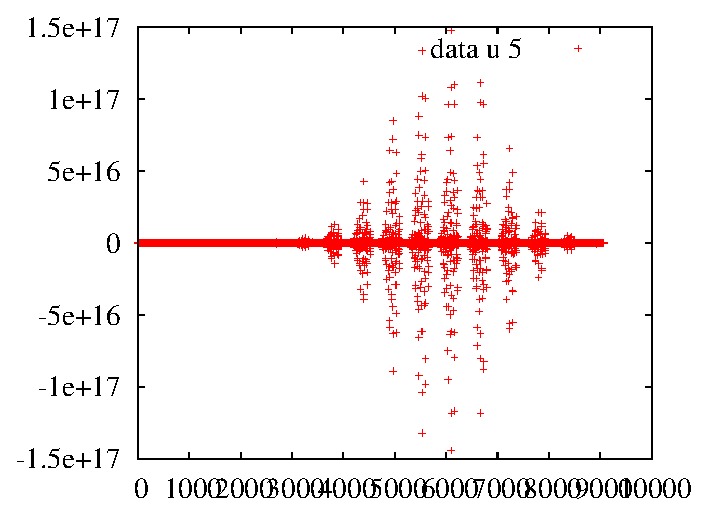
\includegraphics[width=\linewidth]{oscillatoryseries}
\caption{I don't actually remember what bit this is plotting but it's not nice.}
\label{fig:oscillatorysum}
\end{figure}

For completeness, the factors before and after the sum are:

\begin{multline}
A(n,m,n',m',\nu,\mu,\nu',\mu') = \\ \sqrt{\frac{n!}{(m+n)!}} \frac{1}{\sqrt{1+\delta_{m,0}}} \sqrt{\frac{n'!}{(m'+n')!}} \frac{1}{\sqrt{1+\delta_{m',0}}} \\
\sqrt{\frac{ \nu!}{(\mu+\nu)!}} \frac{1}{\sqrt{1+\delta_{\mu,0}}}
\sqrt{\frac{ \nu'!}{(\mu'+\nu')!}} \frac{1}{\sqrt{1+\delta_{\mu',0}}}
\end{multline}

\begin{multline}
B(n,m,k,n',m',k',\nu, \mu,\kappa,\nu',\mu',\kappa') =  \\ 
(-1)^{k} \frac{(n+m)!}{(n-k)!(m+k)!k!}
(-1)^{k'} \frac{(n'+m')!}{(n'-k')!(m'+k')!k'!} \nonumber \\
(-1)^{\kappa} \frac{(\nu+\mu)!}{(\nu-\kappa)!(\mu+\kappa)!\kappa!}
(-1)^{\kappa'} \frac{(\nu'+\mu')!}{(\nu'-\kappa')!(\mu'+\kappa')!\kappa'!}
\\ \eta^{m+m'+2(k+k')} 
\end{multline}

Though these do not help things (B particularly will just make the sum more unwieldy and imprecise).

\subsubsection{Calculating $\intfour$ numerically}

Next we tried to get integrals numerically using NAG routines in Fortran, and also semi-analytically using Wolfram script plugged into the original Fortran code. Both of these examples are available in the modespace folder of code. I compared results obtained with Mathematica, numerically and by sum method above, and found discrepancies even for the best case scenario. The integral doesn't seem well behaved enough to just attack this way.

%%%%%%%%%%%%%%%%%%%%%%%%%%%%%%%%%%%%%%%%%%%%%%%%%%%%%
% REAL SPACE

\pagebreak
\section{EoMs in real space}

\subsection{Dimensionless quantities (lesson learned)}

To make our life simpler having seen the mess of units in the modespace version we define instead dimensionless versions of the quantities in the problem in terms of the beamwaist $w_0/\sqrt{2}$, (where $w_0$ is $w(z_{atoms})$) normalising where necessary. (Note that above we measured instead in the harmonic oscillator length.) We write:

\begin{equation}
\label{eq:fullatomicfield}
\psi(\textbf{r})= \sum_{m,n} \psi_{nm} \  \chi_{n}(x) \chi_m (y)
\end{equation}

and

\begin{multline}
  u_{m,n,q}(x,y,z) = 
  \chi_n (x) \chi_m(y)
  \\
  \cos \left[ f_0 (x,y,z) - \theta_0 (m+n) \right],
\end{multline}

where $\theta_0$ is $\theta(z_{atoms})$ and the $f_0$ term contains all explicitly z-dependent terms which we can integrate as in Sec. \ref{sec:zoverlaps}.

The $\chi$ terms are:

\begin{displaymath}
  \chi_n(x) = \frac{1}{\sqrt[4]{\pi}}
  \frac{1}{\sqrt{2^n n!}} H_n(x) \exp\left(-\frac{x^2}{2} \right).
\end{displaymath}

where the $H_n$ are Hermite polynomials and which yields the orthonormality relation:

\begin{equation}
\label{eq:HGorthonormality}
\int dx \ \chi_n (x) \chi_m (x) = \ \delta_{nm}
\end{equation}

and the completeness relation:

\begin{equation}
\label{eq:HGcompleteness}
\sum_n dx \ \chi_n (x) \chi_n (x') = \ \delta(x-x')
\end{equation}

which mean $\psi$ and $u_{mn}$ are normalised.
We want to introduce an effective transverse light field $\alpha(r)$ which will look something like:

\begin{equation}
\label{eq:fulllightfieldR}
\alpha(\textbf{r})= \sum_{m,n} \alpha_{nm} \  \chi_{n}(x) \chi_m (y)
\end{equation}

\subsubsection{Unitless GPE}

We can rewrite the first two terms of Eq. \ref{eq:eqnpsifirst} in terms of dimensionless units of length, introducing $\eta=\frac{\sqrt(2) \lho}{w_0}$; the $\nabla^2$ term will yield $\left(\frac{\sqrt{2}}{w_0}\right) ^2 \tilde{\nabla}^2$ and the $\textbf{r}^2$ term will yield $\left(\frac{w_0}{\sqrt{2}}\right) ^2 \tilde{\textbf{r}}^2$, where the tilde indicates new dimensionless units.
Therefore, we have:

\begin{equation}
\label{eq:oscillatorpartPsiRealSpace}
- \frac{\hbar \omega_T}{2} 
 \left( \eta^2 \nabla^2-\frac{\textbf{r}^2}{\eta^2}\right) \psi(\textbf{r}) \end{equation}

where $\lho$ is the harmonic oscillator length $\lho=\sqrt{\frac{\hbar}{m_a \omega_T}}$.

We can now divide by $\hbar$ and our $E_0$ will be in terms of frequency (note that were $\mathcal{E}_0 $ was in terms of frequency times area, we now have an $E_0$ in terms of frequency only due to moving to an unitless problem, where effectively we have defined $E_0= \mathcal{E}_0 \left( \frac{\sqrt{2}}{w_0}\right)^2$).

Rewriting the interaction term in the GPE into real-space form, because at the moment it is written in terms of the three-dimensional light field, and doing the z-integral as in Sec. \ref{sec:zoverlaps} we get:

\begin{multline}
i\partial_t \psi(\textbf{r})= ... - E_0 
\sum_{n,m,n',m'} \alpha_{nm}^* \alpha_{n'm'}
 \chi_n (x) \chi_m (y) \\ \chi_{n'} (x) \chi_{m'} (y)
 \frac{1}{4}  \left(e^{i\theta_0(m+n)}e^{-i\theta_0(m'+n')}+h.c. \right)
\psi(\vect{r})
\end{multline}

We multiply both sides by $\int d\textbf{r}' \chi_{nm} (\textbf{r}') \chi_{n'm'} (\textbf{r}')$ and $\int d\textbf{r}'' \chi_{pq} (\textbf{r}'') \chi_{p'q'} (\textbf{r}'')$, where by $\chi_{nm} (\textbf{r})$ we mean $\chi_n(x) \chi_n(y)$; these both yield delta functions from Eq. \ref{eq:HGorthonormality} to detangle the alpha terms from the exponential terms:

\begin{multline}
\label{eq:eqnpsi}
i\partial_t \psi(\textbf{r})= ... - \frac{E_0}{4} \int d\textbf{r}' \int d\textbf{r}''
\sum_{n,m,n',m',p,q,p',q'} \alpha_{nm}^* \alpha_{n'm'} \\
 \chi_{nm} (\textbf{r}') \chi_{pq} (\textbf{r}) \chi_{pq} (\textbf{r}') \chi_{n'm'} (\textbf{r}'') \chi_{p'q'} (\textbf{r}) \chi_{p'q'} (\textbf{r}'') \\
  \left(e^{i\theta_0(p+q+1)}e^{-i\theta_0(p'+q'+1)}+h.c. \right)
\psi(\vect{r})
\end{multline}

We can now use the definition of $\alpha(r)$ from Eq.\ref{eq:fulllightfieldR}.
We also define the function:

\begin{equation}
\label{eq:kernInChis}
K(x,x',\xi)=\sum_{n} \chi_n (x) \chi_n (x') e^{i\xi(n+1/2)}
\end{equation}

which by using Mehler's Kernel

\begin{multline}
\sum_{n}^{\infty} \frac{(\rho/2)^n}{n!} H_n(x) H_n(x') = \\
\frac{1}{\sqrt{1-\rho^2}}
\exp{\left(-
\frac{\rho^2(x^2+x'^2)-2\rho x x'}{(1-\rho^2)}\right)
}
\end{multline}

we can rewrite explicitly in real space:

\begin{multline}
\label{eq:integralkernelK}
K(x,x',\xi)=\sqrt{\frac{1}{i \pi \sin(\xi)}} \\ \exp{\left[ 
\frac{i }{2 } \left(
\frac{x^2+x'^2}{\tan(\xi)}-\frac{2 x x'}{\sin(\xi)}
\right) \right] }
\end{multline}

This makes a lot of sense: this is the harmonic oscillator's Green's Function (or propagator) which encodes propagating the light backwards or forwards by a certain amount of reflections.\\
\\
At this point we should stop to reiterate that we are only working with even modes i.e. for which (m+n) is even; since we've lost the explicit sum to enforce this, we need to insert a similar effect in these kernels.
The full kernel should read:

\begin{multline}
D(\textbf{r},\textbf{r}',\xi)= \sum_{n,m} \frac{1}{2} (1+(-1)^{n+m}) \\ \chi_n (x) \chi_n (x') \chi_m (y) \chi_m (y') e^{i\xi(n+m+1)}
\end{multline}

What we have above yields the term corresponding to the 1 in the round bracket; we also need to build terms corresponding to the Mehler kernels computed with $(-1)^n$ in the definition, which yield a sign change in the $xx'$ term, i.e.:

\begin{multline}
\sum_{n} (-1)^n \chi_n (x) \chi_n (x') e^{i\xi(n+1/2)}= \\\sqrt{\frac{1}{i \pi \sin(\xi)}} \exp{\left[ \frac{i }{2 } \left(
\frac{x^2+x'^2}{\tan(\xi)}+\frac{2 x x'}{\sin(\xi)}  
\right) \right] } =
\\ K(x,-x',\xi)
\end{multline}

So the kernel with the correct parity will read:

\begin{multline}
\label{eq:integralkernelD}
D(\textbf{r},\textbf{r}',\xi)=\frac{1}{2} \big[ K(x,x',\xi)K(y,y',\xi)+ \\ K(x,-x',\xi)K(y,-y',\xi) \big]
\end{multline}


This makes sense; it basically encodes mathematically the fact that, for even order modes, we have mirror image symmetry.
\\
\\
We finally write the last term of the Gross-Pitaevskii equation entirely in real space:

\begin{multline}
i\partial_t \psi(\textbf{r})= ... - \frac{E_0}{4} \\  \int d\textbf{r}' \int d\textbf{r}'' \bigg[
D(\textbf{r},\textbf{r}',\theta_0) \alpha^*(\textbf{r}') \alpha(\textbf{r}'')  D(\textbf{r}, \textbf{r}'',-\theta_0)
+ \\
D(\textbf{r},\textbf{r}',-\theta_0) \alpha^*(\textbf{r}') \alpha(\textbf{r}'')  D(\textbf{r}, \textbf{r}'',\theta_0) \bigg] \psi(\vect{r})
\end{multline}

\subsubsection{Unitless light field equation}

The mode frequency term in real space will be a harmonic oscillator term:

\begin{equation}
-\frac{\nabla^2}{2m_{\alpha}}+ \frac{m_{\alpha} \omega_{\alpha}^2}{2} \vect{r}^2
\end{equation}

From Sec. \ref{sec:modefrequency}, the detuning $\Delta_{nm}=\omega_{nm}-\omega_{pump}$ was defined as $\Delta_{nm}=\Delta_0+(2n+m)\epsilon$, where $\epsilon$ is a `confocality parameter', $\epsilon= \frac{c}{z_M}\left(\psi(z_M)-\frac{\pi}{4}\right)$; the $\Delta_0$ part is independent of n and m, i.e. independent of the basis we're writing things in, therefore simply carries across, whereas the $\epsilon$ acts as our oscillator frequency $\omega_{\alpha}$, so that if the cavity is perfectly confocal the atoms are unbounded.

The oscillator length, in this case our beam waist at the atomic position $ w_0 / \sqrt{2}$, relates to the oscillator quantities:

\begin{equation}
\frac{w_0}{\sqrt{2}}=\sqrt{\frac{1}{m_{\alpha} \epsilon}} \quad \therefore \quad m_{\alpha}=\frac{2}{\epsilon w_0^2}
\end{equation}

In terms of unitless quantities then we have:

\begin{equation}
-\frac{\epsilon}{2} \left[ \nabla^2 - \textbf{r}^2 + \Delta_0 -i\kappa \right] \alpha(\textbf{r})
\end{equation}

The last term then reads, remembering to multiply by $\sum_{nm} \chi_{nm}(r)$ to turn $\alpha_{nm}$ into $\alpha(r)$ and doing the z-integral:

\begin{multline}
i\partial_t \alpha(\textbf{r})= ... - \frac{N E_0}{4}
\sum_{n,m,n',m'} \int d\textbf{r}' |\psi(\textbf{r}')|^2 \chi_{nm} (\textbf{r}) \\
\chi_{nm} (\textbf{r}') \chi_{n'm'}(\textbf{r}')  
\left(e^{i\theta_0(m+n)}e^{-i\theta_0(m'+n')}+h.c. \right) \alpha_{n'm'}
\end{multline}

As above, we introduce the orthonormal expression $\int d\textbf{r}'' \chi_{n'm'}(\textbf{r}'') \chi_{ab}(\textbf{r}'')$ so that we can untangle the indeces in the alpha from the indeces in the exponential:

\begin{multline}
i\partial_t \alpha(\textbf{r})= ... - \frac{N E_0}{4}
\sum_{n,m,n',m',p,q} \int d\textbf{r}' |\psi(\textbf{r}')|^2 \chi_{nm} (\textbf{r}) \\
\chi_{nm} (\textbf{r}') \chi_{n'm'}(\textbf{r}')  \int d\textbf{r}'' \chi_{n'm'}(\textbf{r}'') \chi_{pq} (\textbf{r}'') \alpha_{pq} \\
\left(e^{i\theta_0(m+n)}e^{-i\theta_0(m'+n')}+h.c. \right) 
\end{multline}

Then substituting in the form of $\alpha(r)$ from Eq. \ref{eq:fulllightfieldR} and the integral kernel from \ref{eq:kernInChis}:

\begin{multline}
i\partial_t \alpha(\textbf{r})= ... - \frac{N E_0}{4}
\int d\textbf{r}' \int d\textbf{r}''
\bigg[
D(\textbf{r},\textbf{r}',\theta_0) \\  |\psi(\textbf{r}')|^2 D(\textbf{r}',\textbf{r}'',-\theta_0) +\\
D(\textbf{r},\textbf{r}',-\theta_0)  |\psi(\textbf{r}')|^2 D(\textbf{r}',\textbf{r}'',\theta_0)
\bigg]
\alpha(\textbf{r}'')
\end{multline}

\subsection{Full equations of motion}

We have:


\begin{widetext}

\begin{multline}
\label{eq:realspaceatoms}
i\partial_t \psi(\textbf{r})= - \frac{\omega_T}{2} 
 \left( \eta^2 \nabla^2-\frac{\textbf{r}^2}{\eta^2}\right) \psi(\textbf{r}) + UN |\psi(\textbf{r})|^2- \frac{E_0}{4}  \bigg[ \abs*{ \int d\textbf{r}' D(\textbf{r}, \textbf{r}',\theta_0) \alpha(\textbf{r}')} ^2+\abs*{\int d\textbf{r}' D(\textbf{r},\textbf{r}',-\theta_0) \alpha(\textbf{r}')}^2 \bigg] \psi(\vect{r})
\end{multline}

and 

\begin{multline}
\label{eq:realspacelight}
i\partial_t \alpha(\textbf{r})=  \left[ -\frac{\epsilon}{2} \left( \nabla^2 - \textbf{r}^2 \right) + \Delta_0 -i\kappa \right] \alpha(\textbf{r}) + f_p(\textbf{r})- \frac{N E_0}{4}
 \int d\textbf{r}'\int d\textbf{r}'' \bigg[ D(\textbf{r},\textbf{r}'',\theta_0) |\psi(\textbf{r}'')|^2  D(\textbf{r}',\textbf{r}'',-\theta_0)  + h.c.\bigg]\alpha(\textbf{r}')
\end{multline}
\end{widetext}

Where the wavefn of the atoms is normalised to one and we have included an atom-atom interaction term $UN |\psi(\textbf{r})|^2$ as well.

This means we really only need to compute three integrals, $D(\textbf{r},\textbf{r}',\theta_0)*\alpha(\textbf{r}')$, $D(\textbf{r},\textbf{r}',-\theta_0)*\alpha(\textbf{r}')$ and the light field interaction term $X(\textbf{r},\textbf{r}'')*\alpha(\textbf{r}'')$ where we have rolled up the inner integral into the term $X(\textbf{r},\textbf{r}'')= D(\textbf{r},\textbf{r}',\theta_0)*|\psi(\textbf{r}')|^2*D(\textbf{r},\textbf{r}',-\theta_0)$. This, however, can be simplified into alpha integrals which we have already computed for the atomic equation of motion, and then doing the second integral.
 
This last term looks like the more troublesome term, so we will use it as a meter to gauge whether the numerics have sufficient resolution. 

\subsection{Periodicity of the equations of motion}

Given that we are in a confocal or near-confocal cavity, we'd normally expect the equations of motion to have a $2 \pi$ periodicity (four round trips to come back to itself, which makes sense given $0<\theta_0<\pi/2$); however, given that we take only even order modes which have, as observed above, mirror image symmetry in the transverse plane, the effective symmetry of the equations should be $\pi$ s.t. $\pi-\theta=\theta$.

The parameter that governs the phase accumulation (and therefore the z-position dependent term in the now transversal EoMs) appears in the exponential term:

\begin{equation}
e^{i \theta_0 (m+n-m'-n')}+e^{-i \theta_0 (m+n-m'-n')}
\end{equation}

which is periodic in $\pi$, just as the combination of two integral kernels that include this:

 \begin{figure}[H]
  \centering
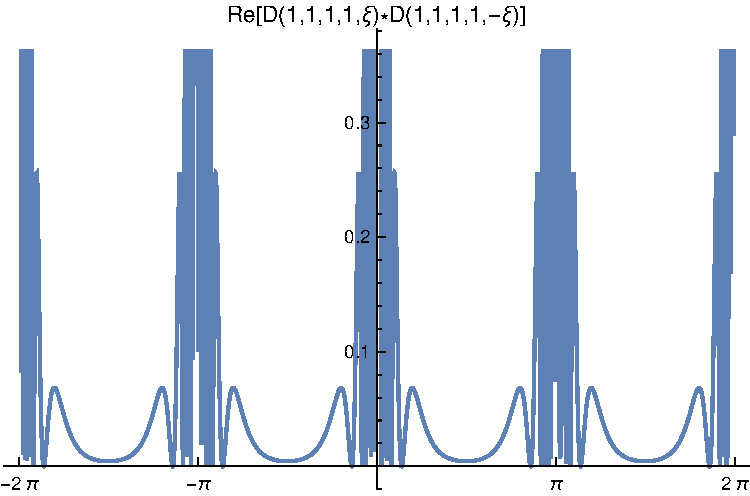
\includegraphics[width=\linewidth]{periodicityKernels}
\caption{Periodicity of the combination of two integral kernels, which are what appears in the EoMs.}
\end{figure}

Note that a single integral kernel does not have this periodicity:

\begin{figure}[H]
\centering
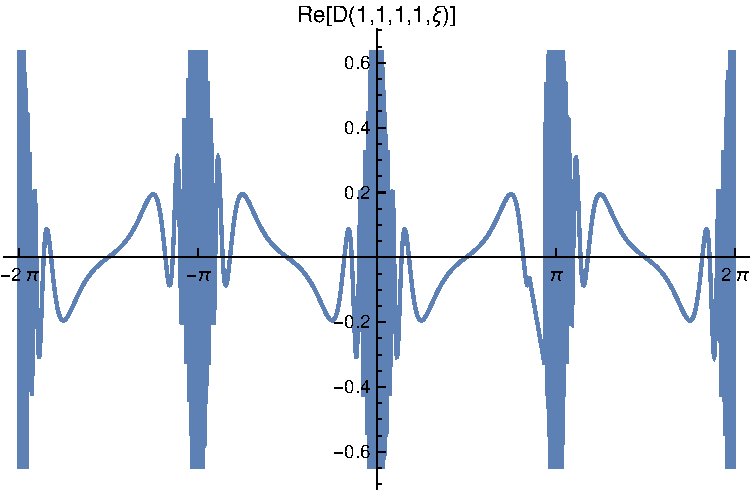
\includegraphics[width=\linewidth]{periodicityKernel}
\caption{Periodicity of a single integral kernel.}
\end{figure}

This makes sense -- consider the (quantum) harmonic oscillator $e^{i\omega(n+1/2)}$ with $n=2N$; this yields a part which is periodic in $\pi$ and a part that isn't due to the $1/2$ factor (zero point energy). This is just a phase factor so it doesn't influence the observable behaviour, but it does mean that technically the wavefunction only comes back to itself exactly afer $2 \pi$. The same thing is happening in the integral kernels, which makes sense as they are the harmonic oscillator Green's functions.
The kernels never appear on their own in the equations of motion.

\subsection{Introducing higher order mode suppression}

If one goes to model the full light field as above, one finds that the oscillations due to keeping all modes make the problem numerically intractable, so we're going to introduce a higher order cutoff in the hopes to make the oscillations better behaved.
The place to do this is in \ref{eq:kernInGreens}, where we redefine $\xi\rightarrow\xi+i\gamma$ to include an exponential decay term as a function of mode order $\exp{-\gamma(n+m+1)}$ so that:

\begin{multline}
K_{cutoff}(x,x',\xi)=\sqrt{\frac{1}{i \pi \sin(\xi+i \gamma)}} \\\ \exp{\left[ 
\frac{i}{2} \left(
\frac{x^2+x'^2}{\tan(\xi+i \gamma)}-\frac{2 x x'}{\sin(\xi+i \gamma)}
\right) \right] }
\end{multline}

And 

\begin{multline}
D_{cutoff}(\textbf{r},\textbf{r}',\xi+i \gamma)=\\ \frac{1}{2} \big[ K(x,x',\xi+i \gamma)K(y,y',\xi+i \gamma)\\+ K(x,-x',\xi+i \gamma)K(y,-y',\xi+i \gamma) \big]
\end{multline}

This effectively means that we only keep lower order modes, e.g. for a factor of $\gamma=1/50$ we only have contributions from the first 50 modes, which will suppress the oscillations at higher x in the kernel, making it more tractable.

We can then try to sample the new convolution $X_{cutoff}(r,r'')=D_{cutoff}(r',r'',\xi) * |\psi(r')|^2 * D_{cutoff}(r,r',-\xi)$ discretely, using dummy light and atomic field functions with gaussian peaks where necessary, and compare this to the continuous result to establish a reasonable grid spacing to run XMDS with to capture the full detail.


\subsubsection{Feature width and effect on sampling}

The width of the features of $X_{cutoff}$ is determined by the width of the features in the atomic field. There are two problems with this: on the one hand, if the features of the wavefunction get too fine, $X_{cutoff}$ gets more oscillatory, so there are more features to captura (a small gaussian only 'smooths' the oscillatory kernels on a shorter range); on the other the kernel convolution acts like a FT, yielding narrower peaks for wider wavefunction, so we need a fine enough grid to capture this.

\begin{figure}[t]
  \centering
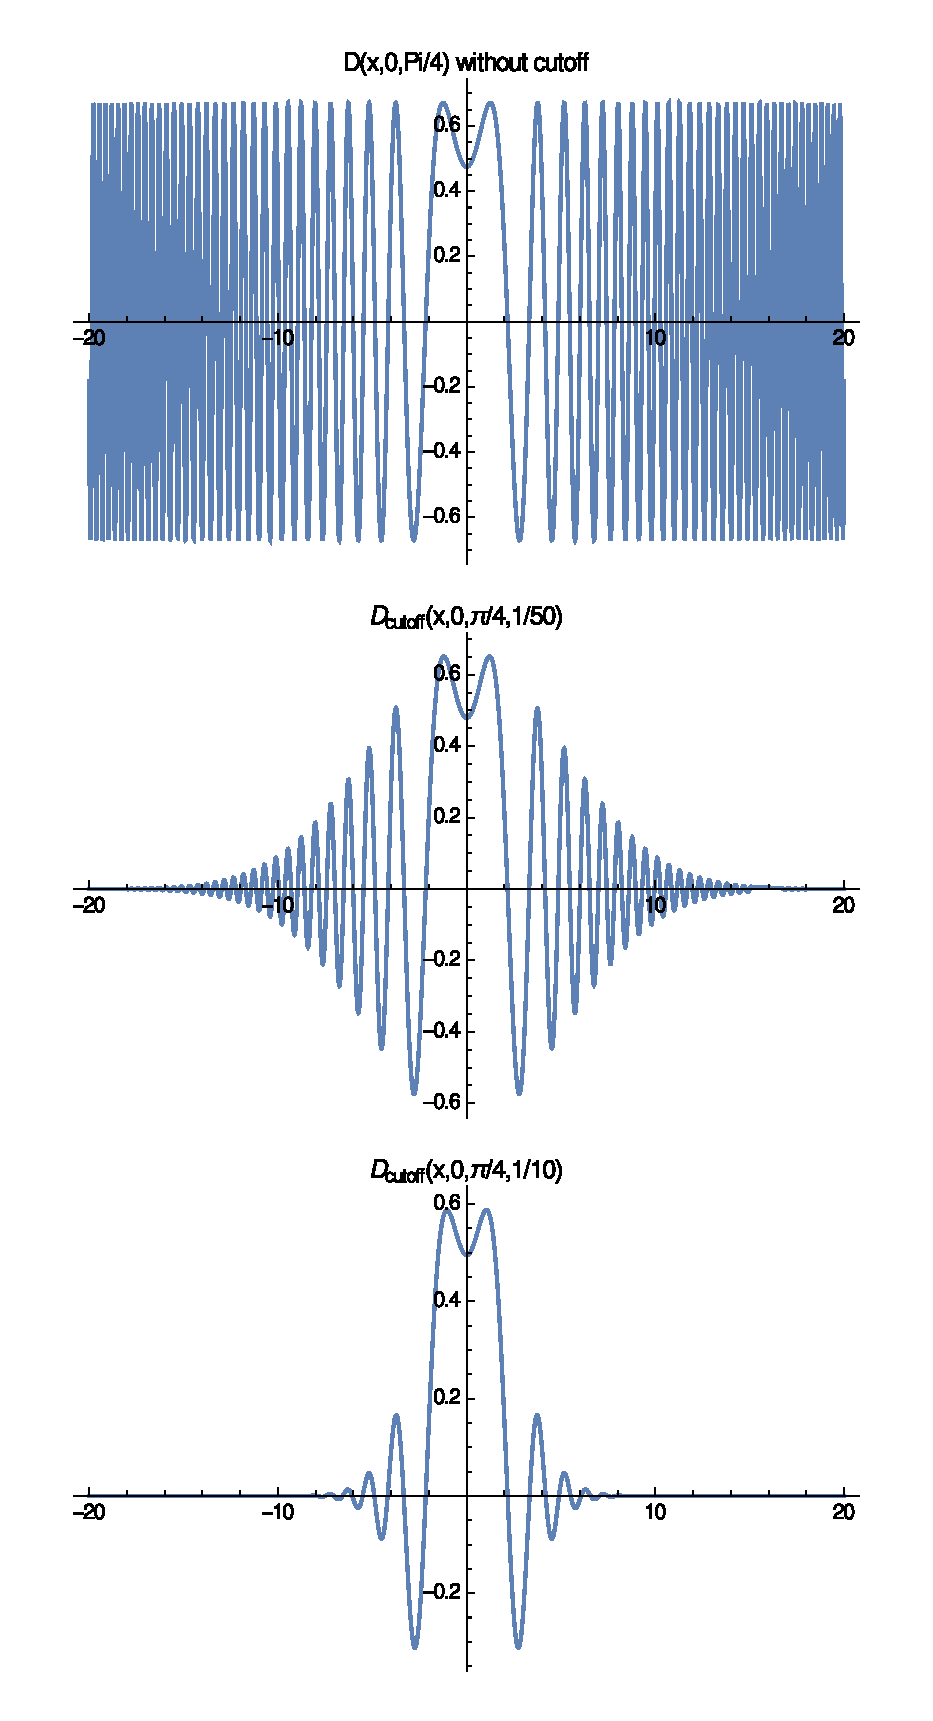
\includegraphics[width=\linewidth]{debugging/kernelcutoffs}
\caption{\textbf{\textbar~ Integral kernels with cutoffs:} Plotting (a) including all modes (b) keeping the first ~50 modes (c) keeping the first ~10 modes.}
\end{figure}

It makes sense to use an atomic cloud size of roughly the same size as the `multimode beam waist' defined by the kernel cutoff i.e. atomic cloud of sufficient size to interact with all modes. Can define roughly $\sigma=\sqrt{modes/4}$, i.e. if we want to keep 20 modes, we'll have $D_{cutoff}(x,x',\xi,1/20)$ and the atomic field and therefore its features will be at most of width $\psi=\frac{\exp \left(-\frac{(x-x_0)^2}{40}\right)}{\sqrt[4]{10\pi }}$:

\begin{figure}[H]
  \centering
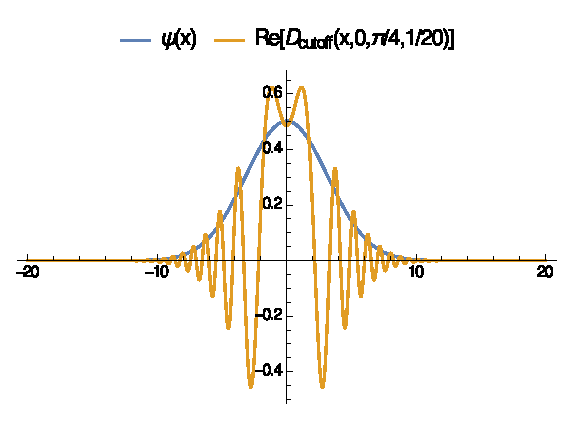
\includegraphics[width=\linewidth]{debugging/psiandkern}
\caption{\textbf{\textbar~ Dummy psi and kernel} with matching cutoff and therefore width (keeping 20 modes).}
\end{figure}

We will use this in figuring out an upper limit of modes we can keep (how oscillatory the kernel can be while still yielding the right result when sampled discretely on a reasonable grid). We should also bear in mind that very small real-space features might give problems, i.e. check how small we can make $\sigma$ and still obtain a sensible discretised $X_{cutoff}$.
\\

[Sanity-check: the x axis is really dimensionless $\tilde{x}=x/(w_0/\sqrt{2})$ where $w_0$ is the zeroth mode beam waist. If one sets $\gamma=1$ (i.e. keeping one mode) the kernel is indeed a gaussian of width $w_0/\sqrt{2}$ (or at least something that looks sensible in that way).] 

\subsubsection{Sampling features}

\begin{figure}[H]
  \centering
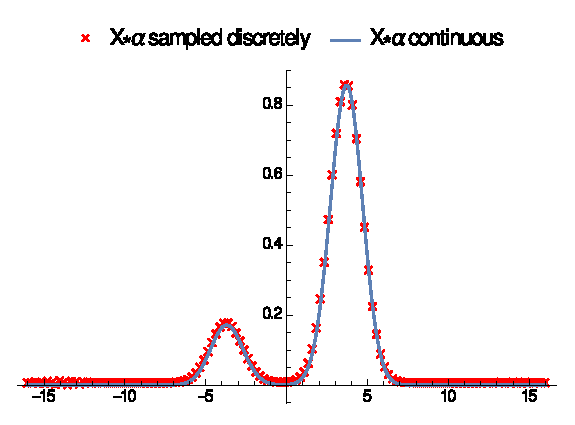
\includegraphics[width=\linewidth]{debugging/Xalpha50modes128grid}
\caption{Keeping 50 modes, 128 points grid, \{-16,16\}.}
\end{figure}

\begin{figure}[H]	
  \centering			
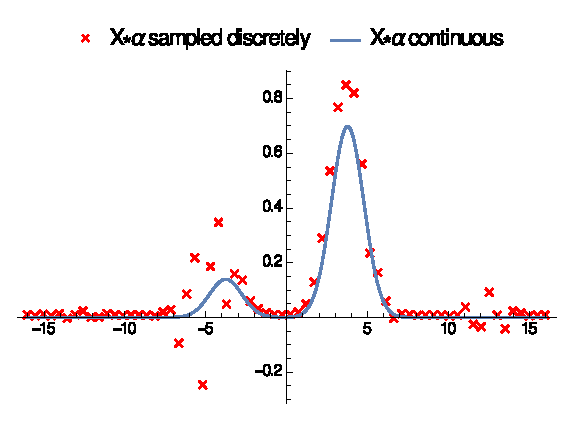
\includegraphics[width=\linewidth]{debugging/Xalpha50modes64grid}
\caption{Keeping 50 modes, 64 points grid, \{-16,16\}.}		
\end{figure}

\begin{figure}[H]	
  \centering			
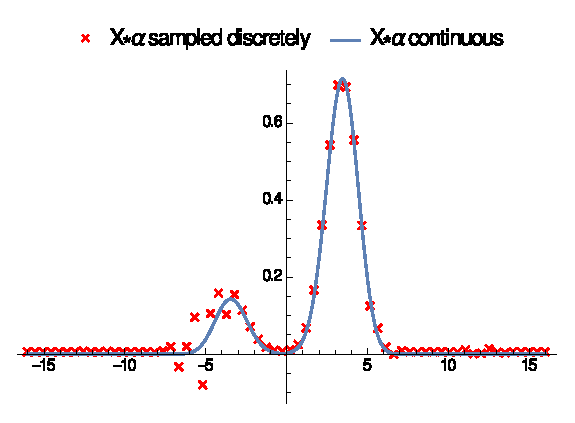
\includegraphics[width=\linewidth]{debugging/Xalpha25modes64grid}
\caption{Keeping 25 modes, 64 points grid, \{-16,16\}.}
\end{figure}

\begin{figure}[H]	
  \centering			
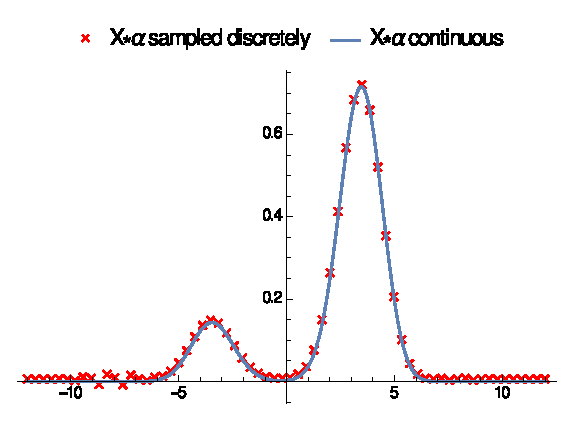
\includegraphics[width=\linewidth]{debugging/Xalpha25modes64grid12to12}		
\caption{Keeping 25 modes, 64 points grid, \{-12,12\}.}
\end{figure}

\begin{figure}[H]	
  \centering			
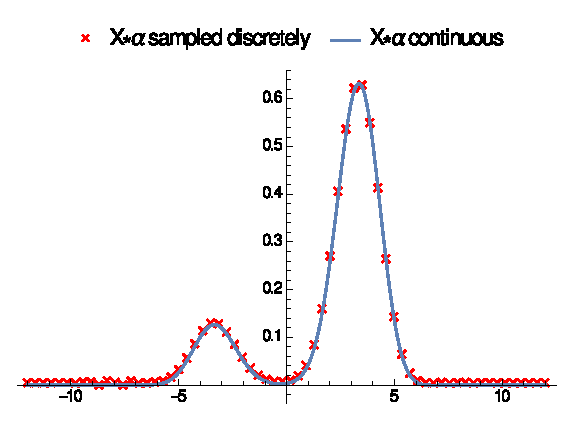
\includegraphics[width=\linewidth]{debugging/Xalpha20modes64grid}		
\caption{Keeping 20 modes, 64 points grid, \{-12,12\}.}
\end{figure}

\subsection{Interaction term in Fourier space}

Two reasons to want k-space forms: 
\begin{itemize}
	\item \textcolor{cyan}{ previously: the full code at several (should-be) simple stages outputs a bizarre light field profile even for short times after pumping is turned on; the light field does seem to grow linearly in time and then saturate but we could get some insight into what's happening;}
	\item but mostly: if we find that the $k, k'$ dependent interaction term can be written as a function of $k-k'$ only (or as a function only weakly dependent on $k+k'$) we can rewrite this in a single coordinate and therefore do away with the aliasing.
\end{itemize}

To do this we can attempt to simplify the light field equation by assuming the pump spot and atomic field distribution are Gaussian where relevant, which is reasonable at short times as we initialise both of these as Gaussian; we can then rewrite the EoM in k-space where the interaction term might be local, and see what the analytic forms tell us.
\\
It turns out that FTing the $D(\textbf{r},\textbf{r}',\xi)$ doesn't particularly help. In 1D:

\begin{multline}
D(k_x,k_{x}',\xi)=\int \frac{d x}{\sqrt{2 \pi}} \int \frac{d x'}{\sqrt{2 \pi}} e^{i (k_x x + k_{x}' x')} D(x,x',\xi)
\end{multline}

Since the D's are dimensionless, carrying out x and x' integrals, one gets back to:

\begin{equation}
D(k_x,k_{x}',\xi)=\sqrt{\frac{1}{i \pi \sin{\xi}}} \exp{\left[ \frac{i }{2 } \left(
\frac{k_x^2+k_x'^2}{\tan(\xi)}-\frac{2 k_x k_x'}{\sin(\xi)}  
\right) \right] } 
\end{equation}

SPOILER - The analytics tell us we do indeed expect a much more regular behaviour, and these must be artefacts; we therefore look to simplify the problem somehow so that it's easier to handle for the numerics.

--

We can consider the atomic field eqn in k-space entirely. We want to multiply both sides of the equation by the inverse FT terms to get eqn of motion for $\psi(k)$:

\begin{equation}
\psi(\textbf{k})= \int d\textbf{r} \  e^{i\textbf{k} \textbf{r}} \psi(\textbf{r})
\end{equation}

So we need to contend with the two mod-squared terms. Thinking about one of them:

\begin{equation}
  \abs*{ \int d\textbf{r}' D(\textbf{r}, \textbf{r}',\theta_0) \alpha(\textbf{r}')} ^2 \psi(\textbf{r})
\end{equation}


FTing the content of the mod-sq:


\begin{multline}
\int d \textbf{r}' \int \frac{d \textbf{k}}{2 \pi} \int \frac{d \textbf{k}'}{2 \pi} D(\textbf{k},\textbf{k}',\theta_0) e^{-i (\textbf{k} \textbf{r}+\textbf{k}' \textbf{r}')} \\ \int \frac{d \textbf{k}''}{2 \pi} e^{-i \textbf{k}'' \textbf{r}'} \alpha(\textbf{k}'')
\end{multline}

(NB this is *just* the stuff inside the abs val)

The $\textbf{r}'$ integral yields $2 \pi \delta(\textbf{k}'+\textbf{k}'')$, so we get:

\begin{multline}
\int \frac{d \textbf{k}}{2 \pi} \int \frac{d \textbf{k}'}{2 \pi} D(\textbf{k},\textbf{k}',\theta_0) e^{-i \textbf{k} \textbf{r}} \alpha(-\textbf{k}')
\end{multline}

and likewise for the complex conjugate in another set of momenta. To obtain the equations of motion we then have:

\begin{multline}
i \partial_t \psi(\textbf{p})=...+\frac{E_0}{4}\int d\textbf{r} \
\psi(\textbf{r}) e^{-i (\textbf{k}+\textbf{q}-\textbf{p})\textbf{r}} \\
 \int \frac{d \textbf{k}}{2 \pi} \int \frac{d \textbf{k}'}{2 \pi}
\int \frac{d \textbf{q}}{2 \pi} \int \frac{d \textbf{q}'}{2 \pi}  D(\textbf{k},\textbf{k}',\theta_0) D(\textbf{q},\textbf{q}',-\theta_0) \\  \alpha(-\textbf{k}') \alpha^*(-\textbf{q}') 
\end{multline}

which yields

\begin{multline}
i \partial_t \psi(\textbf{p})=...+\frac{E_0}{4}
 \int \frac{d \textbf{k}}{2 \pi} \int \frac{d \textbf{k}'}{2 \pi}
\int \frac{d \textbf{q}}{2 \pi} \int \frac{d \textbf{q}'}{2 \pi}  \\ D(\textbf{k},\textbf{k}',\theta_0) D(\textbf{q},\textbf{q}',-\theta_0) \\  \alpha(-\textbf{k}') \alpha^*(-\textbf{q}') \psi(\textbf{p}-\textbf{k}-\textbf{q})
\end{multline}

Not particularly helpful.


\subsection{Solving 1D problem for rotationally symmetric ground state}

We can simplify the problem by deriving effectively one-dimensional equations for a rotationally symmetric steady state (i.e. in r only), to which we can then introduce perturbations in the angular dimension. Given that the code includes aliases, this would bring us down from four dimensions to two which with power law time evo (?) should speed us up a lot.

To derive this, we assume that that the light field and the atomic field have no angular dependence, i.e. $\psi(\textbf{r})=\psi(r,\theta)=\psi(r)$ and  $\alpha(\textbf{r})=\alpha(r,\theta)=\alpha(r)$. We also assume the pump is rotationally symmetric.
Note that the atomic wavefunction is still normalised in two dimensions, i.e.

\begin{equation}
\int_{0}^{2 \pi} d \theta \int_0^{\infty} r dr |\psi(\textbf{r})|^2=1
\end{equation}

so the 1D version in the code won't be by a factor of $1/2\pi$.

We want to write out Eq.\ref{eq:realspaceatoms} and Eq.\ref{eq:realspacelight} in $r,\theta$ and then integrate out $\theta$ (picking up factors of $2\pi$ where the integration is trivial, since we've assumed the wavefunctions have no angle dependence). For example with the light equation:

\begin{multline}
\label{eq:integrateouttheta}
i 2 \pi \partial_t \alpha(r)= 2\pi \left[ -\frac{\epsilon}{2} \left( \nabla^2 - r^2 \right) + \Delta_0 -i\kappa \right] \alpha(r)\\ +2\pi  f_p(r)- \frac{E_0}{4}
\int d\theta \int d\theta'\int d\theta'' \int dr'\int r'' \\ \bigg[ D(\textbf{r},\textbf{r}'',\theta_0) |\psi(r'')|^2  D(\textbf{r}',\textbf{r}'',-\theta_0)  + h.c.\bigg]\alpha(r')
\end{multline}

So this becomes a matter of figuring out what becomes of the integral kernels (for a change...?).
Writing Eq.\ref{eq:integralkernelK} and Eq.\ref{eq:integralkernelD} in $r,\theta$:

\begin{multline}
D(\textbf{r},\textbf{r}',\xi)=\frac{1}{2}\frac{1}{i \pi \sin(\xi)}  
\exp{\left( \frac{i }{2\tan(\xi) } 
(|\textbf{r}|^2+|\textbf{r}'|^2) \right)}
\\ \bigg[
\exp{ \left(
\frac{i }{\sin(\xi)} |\textbf{r}|\cdot|\textbf{r}'|
\right)
}
+
\exp{ \left(
-\frac{i }{\sin(\xi)} |\textbf{r}|\cdot|\textbf{r}'|
\right)
}
\bigg]=\\
\frac{1}{2 i \pi \sin(\xi)}  
\exp{\left( \frac{i }{2\tan(\xi) } 
(r^2+r'^2) \right)}
\\ \bigg[
\exp{ \left(
\frac{i }{\sin(\xi)} r r' \cos(\theta-\theta')
\right)
}
+
\exp{ \left(
-\frac{i }{\sin(\xi)} r r' \cos(\theta-\theta')
\right)
}
\bigg]
\end{multline}

Integrating the angular part of this in $\theta'$ per equation of motion yields $ 4 \pi J_0\left( \frac{r r'}{\sin(\xi)}\right)$ (the factor of 2 is from the two terms symmetrising the kernel).

So we define a new angle-independent integral kernel:

\begin{multline}
D_{rot}(r,r',\xi)=\frac{2}{i \sin(\xi)} J_0\left( \frac{r r'}{\sin(\xi)} \right)  \\
\exp{\left( \frac{i }{2\tan(\xi) } 
(r^2+r'^2) \right)}
\end{multline}

And the equation of motion then reads:

\begin{multline}
i \partial_t \alpha(r)= \left[ -\frac{\epsilon}{2} \left( \nabla^2 - r^2 \right) + \Delta_0 -i\kappa \right] \alpha(r)\\ + f_p(r)- \frac{E_0}{4}
 \int dr'\int r'' \\ \bigg[ D_{rot}(r,r'',\theta_0) |\psi(r'')|^2  D_{rot}(r',r'',-\theta_0)  + h.c.\bigg]\alpha(r')
\end{multline}

purely in the radial dimension.

Similarly, for the atomic field:



%%%%%%%%%%%%%%%%%%%%%%%%%%%%%%%%%%%%%%%%%%%%%%%%%%%%%
% APPENDIX CONTENT

\appendix

\section{Normalisation of $\alpha(\vect{r})$ and $u_{nm}$}
\label{sec:normalisation-from-HG}

Using orthonormality of Hermite polynomials:

\begin{equation}
\int_{- \infty}^{\infty} dx H_n(x) H_m(x) e^{-x^2}=\sqrt{\pi} 2^n n! \delta_{nm}
\end{equation}

ones gets:

\begin{equation}
\int dx \ \chi_n \left(\frac{\sqrt{2}x}{w_0}\right) \chi_m \left(\frac{\sqrt{2}x}{w_0}\right) = w_0 \ \delta_{nm}
\end{equation}

and therefore both $\alpha(x,y)$ and the $u_{nm}$ are normalised.

Similarly for Laguerre-Gauss:

\begin{equation}
\label{eq:LGorthonorm}
\int_0^\infty \mathrm{d}x \ e^{-x} \ x^k \ L^k_n(x) \ L^k_m(x) = \frac{n+k!}{n!} \delta_{n,m}
\end{equation}

But in this case the Laguerre terms are in terms of $\frac{r^2}{\lho}$, so we need to transform variables to obtain the result:

\begin{equation}
\label{eq:Chiorthonorm}
\int \mathrm{d}r \ \chiaf \chi_{\nu',\mu}^L\left(\frac{r}{\lho}\right) = \frac{\lho^2}{\pi} \  \delta_{\nu,\nu'}
\end{equation}

\section{Gaussian optics notes}
\label{sec:gaussian-optics}

From Siegmann, the complex beam propagation function $\tilde{q}(z)$
obeys
\begin{displaymath}
  \frac{1}{\tilde{q}{z}} = \frac{1}{R(z)} - \frac{2 i}{k w(z)^2}
\end{displaymath}
and $\tilde{q}(z) = z + i z_R$ (possibly with a real shift).  This gives
\begin{displaymath}
  R(z) = z + \frac{z_R^2}{z}, \quad
  w(z) = w_0 \sqrt{ 1 + \frac{z^2}{z_R^2}}
\end{displaymath}
where $z_R = k w_0^2/2$, or equivalently, $w_0 =\sqrt{\lambda
  z_R/\pi}$.  For the symmetric confocal cavity, we have mirrors with
radius of curvature $\pm 2 z_R$ placed at $z=\pm z_R$.  

The Guoy phase is given in general by 
\begin{displaymath}
  \tan(\psi(z)) = \frac{k w(z)^2}{2R(z)}
\end{displaymath}
or, more usefully, $\psi(z) = \arctan(z/z_R)$.  In the confocal
case, it thus runs between $\pm \pi/4$.

If we consider the general $z$ dependent standing wave:
\begin{displaymath}
  \cos\left[ k \left( z + \frac{r^2}{2R(z)} \right)
    - (m+n+1) \psi(z) + \xi_{m,n,q} \right],
\end{displaymath}
then boundary conditions impose that this argument must be $\pi/2$ at
one end of the cavity, and $(q+1/2) \pi$ at the other --- i.e. there
must be $q$ multiples of $2\pi$ in a complete round trip.  This gives
the conditions:
\begin{displaymath}
  \xi = \frac{\pi}{2}(q+1), \quad
  2kz_0 = \frac{\pi}{2} \left[ 2q + (m+n+1) \frac{4\psi(z_0)}{\pi} \right].
\end{displaymath}

given that on the mirrors $z=-z_1+\frac{r^2}{2|R_m|}$ and $z=z_1-\frac{r^2}{2|R_m|}$; $R(z_1)=|R_m|$,  $R(-z_1)=-|R_m|$ at $z_R$; and in general $\psi(-z)=\psi(z)$.\\
For the confocal case, families of degenerate modes obey
$2q + m + n = 2 q_0$, where the label $q_0$ of the fundemental
mode is related to the wavevector by
$\omega = c k = c\pi (2q_0 +1) / 4 z_0$.  In this case we may then label
$\xi_{m,n,q} = \xi_{m,n,q_0} = \xi_{q_0} - (m+n)\pi/4$.  It is therefore
convenient to write the mode as:
\begin{displaymath}
  \cos\left[ k \left( z + \frac{r^2}{2R(z)} \right)
    + \xi_{q_0} - \psi(z)
    - (m+n) \left( \frac{\pi}{4} + \psi(z) \right)
  \right],
\end{displaymath}
which identifies clearly that the $m,n$ phase dependence involves the
combination $\theta(z)=\psi(z) + \pi/4$, which goes between $0$ and $\pi/2$.
The cos term can therefore be rewritten for convenience as 

\begin{displaymath}
\label{eq:costermdivisible}
\cos[f_0(\vect{r},z)-\theta(z)(m+n)]
\end{displaymath}

containing an m,n-independent term $f_0(\vect{r},z)$ and a m,n-dependent term multiplying $\theta(z)$.

\end{document}